\section{Imaging System Parameters}

The design of the sensor includes selection of three important parameters: the aperture diameter $D$, the focal length $z$ and the wavelength $\lambda$.  To see how changing these parameters will influence the image quality we can look at the point spread functions (PSF), but, first, it may be useful to consider the Rayleigh Criterion.

\subsection{Rayleigh Criterion}
To see the effect of the imaging system on the Fraunhofer diffraction patterns discussed up to this point, the system resolution can be determined.  The Rayleigh Criterion assesses the quality of an optical system in terms of its resolution - how close two points can be while still being able to be identified separately - for the limiting case of a circular aperture.  It is given in Equation \ref{RayleighC}.

\begin{equation}
\label{RayleighC}
	 \Delta \ell = 1.220 \frac{ f \lambda}{D}.
\end{equation}

In this equation, $\Delta \ell$ is the spatial resolution of the system, $f$ is the focal length, $\lambda$ is the wavelength of the light and $D$ is the diameter of the aperture.  The Rayleigh criterion is derived directly from the expression of the PSF.  Rayleigh proposed that two sources could be distinguished from one another if their separation was sufficient that the position of their maximum intensities were at least $\Delta \ell$ apart.  This distance is the spacing between two peaks when the intersection of two PSFs is at half of the maximum intensity of each of the sources. This is illustrated in Figure \ref{fig:Rayleigh} where as two sources move closer together they shift from being easy to identify separately to appearing as a single source.

\begin{figure}[H]
	\centering
		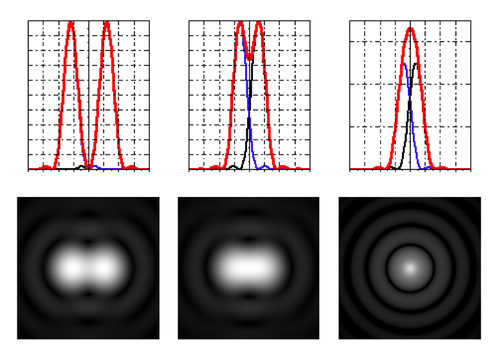
\includegraphics[width=1.0\textwidth]{figures/RayleighCriterion.png}
	\caption{Rayleigh Criterion: (a) PSF for two easily resolved sources, (b) PSF for two just resolvable sources, (c) PSF for two unresolvable sources. }
	\label{fig:Rayleigh}
\end{figure}

%image source: http://pinholeworks.com/wp/goerge-airy-vs-lord-rayleigh/

To reduce the resolution the system is limited to, a thin PSF is desirable.  The equation for Rayleigh's criterion shows that this can be varied by selecting the aperture diameter (typically the lens diameter), the focal length and the wavelength of the light.  

\subsection{Varying System Parameters}
Increasing the diameter of the aperture, increasing the focal length or increasing the wavelength will all decrease the diffraction of the system.  The following PSFs show the results of these changes while holding all other parameters constant.  

\begin{figure}[H]
	\centering
		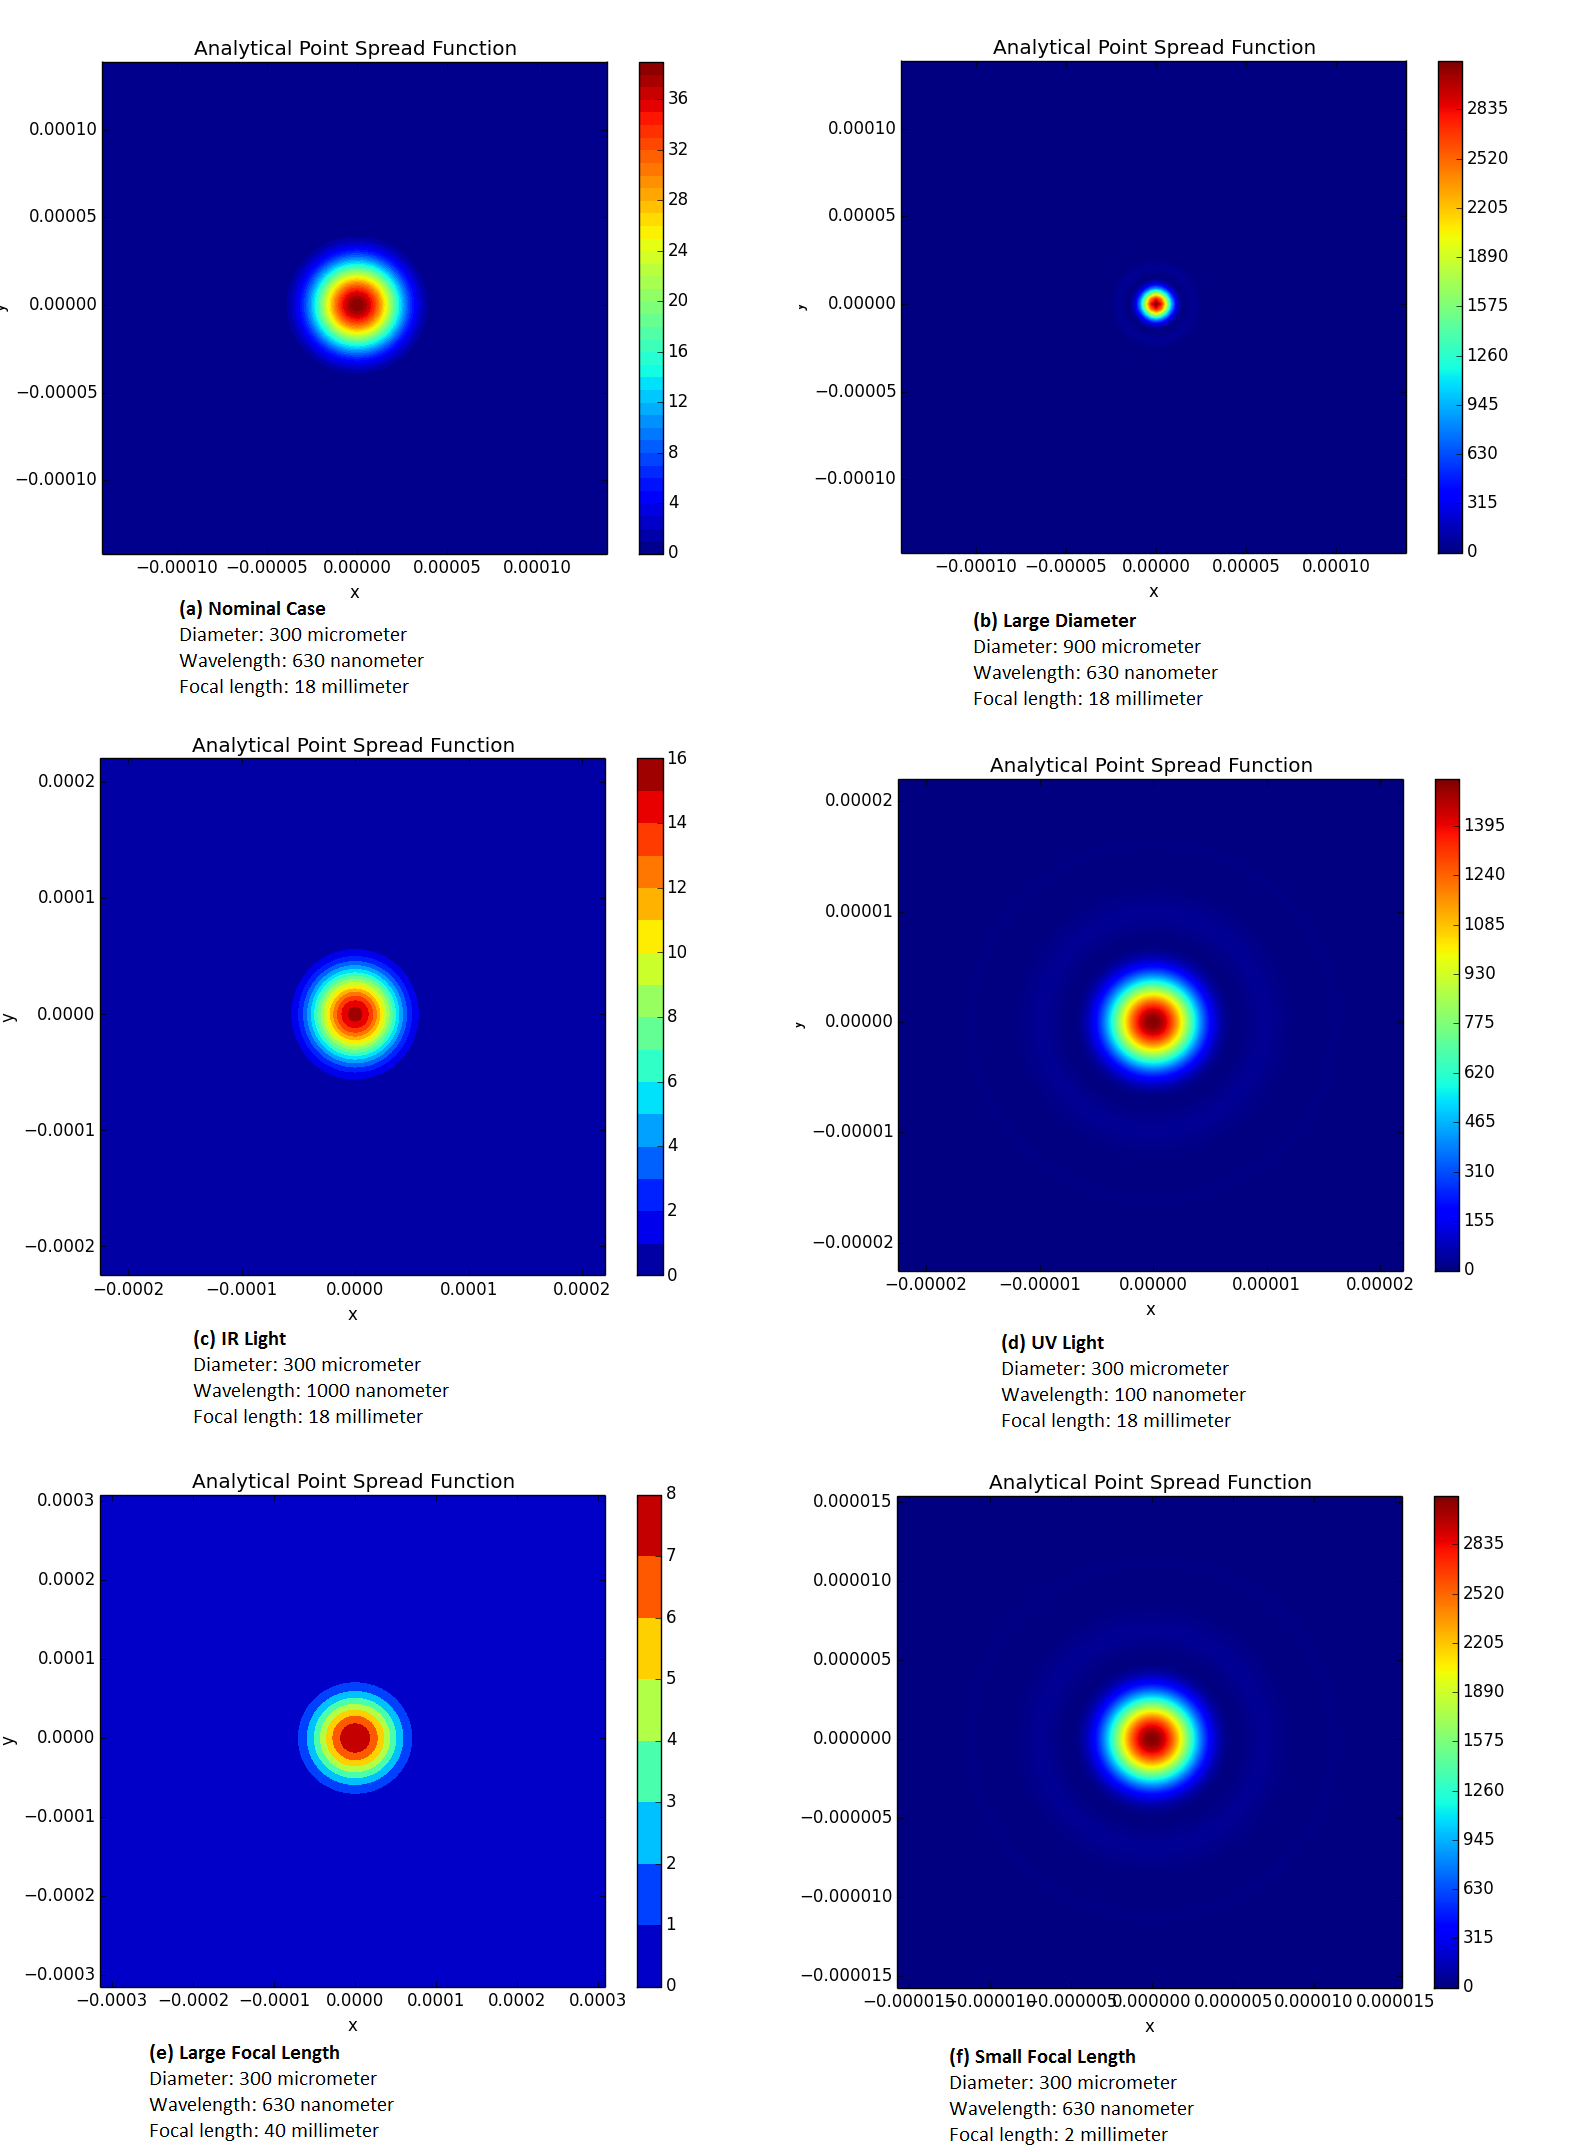
\includegraphics[width=1.0\textwidth]{figures/VarySysParams.png}
	\caption{PSF for various values of aperture diameter, wavelength and focal length. }
	\label{fig:VaryParams}
\end{figure}


